\begin{table}[htbp]
\centering
\small
\caption{Grouped reported-rank percentile curves. Each figure overlays one protein system and sampling scheme, with reported cohorts in separate panels.}
\label{tab:reported-curves-index}
\begin{tabular}{llrr}
\toprule
Scheme & Family & Analyses & Figures \\
\midrule
Parameter & PDZ & 14 & \ref{fig:curves-parameter_posterior-pdz-1} \\
Parameter & TrpB & 28 & \ref{fig:curves-parameter_posterior-trpb-1} \\
Parameter & NucB & 7 & \ref{fig:curves-parameter_posterior-nuc-1} \\
Optimized-fit counts & PDZ & 19 & \ref{fig:curves-mle_predictive-pdz-1} \\
Optimized-fit counts & TrpB & 34 & \ref{fig:curves-mle_predictive-trpb-1} \\
Optimized-fit counts & NucB & 7 & \ref{fig:curves-mle_predictive-nuc-1} \\
Posterior counts & PDZ & 14 & \ref{fig:curves-posterior_predictive-pdz-1} \\
Posterior counts & TrpB & 28 & \ref{fig:curves-posterior_predictive-trpb-1} \\
Posterior counts & NucB & 7 & \ref{fig:curves-posterior_predictive-nuc-1} \\
\bottomrule
\end{tabular}
\end{table}
\clearpage

\begin{figure}[p]
\centering
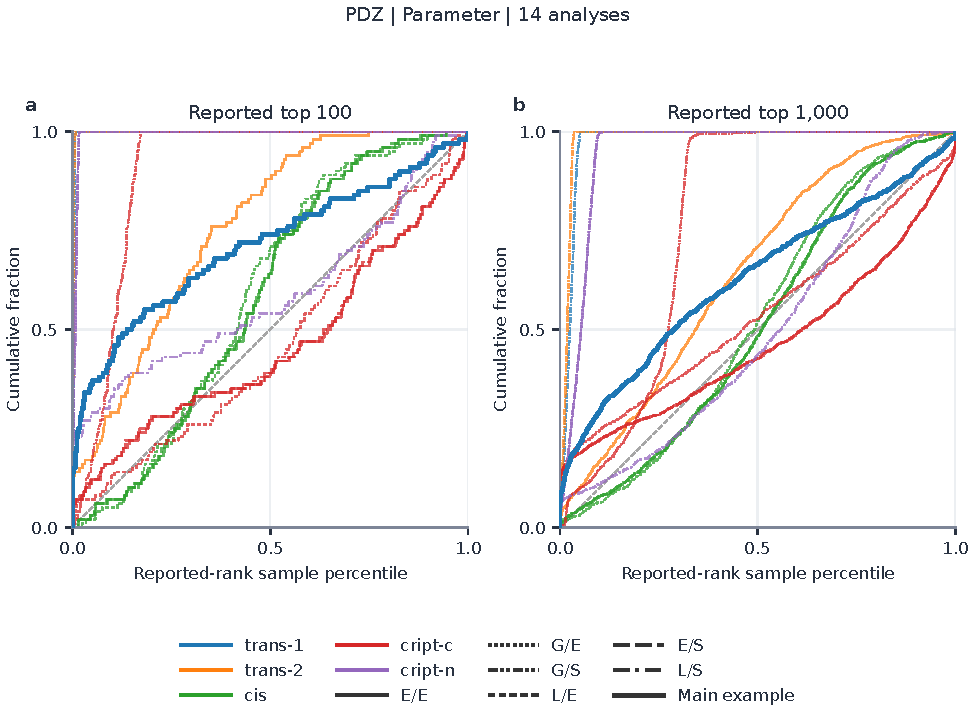
\includegraphics[width=\linewidth]{reported_curves_parameter_posterior_pdz_01.pdf}
\caption{PDZ reported-rank percentile curves: parameter. Each of the 14 lines per panel is one landscape/model analysis; panels use the reported top 100 and top 1000. Colors identify landscapes and line styles identify models. E, L, and G denote Exponential, Lomax, and Gamma priors; a second E or S denotes exponential or sigmoid growth. A thicker line marks the main example. All percentiles are retained; curves are overlaid, not averaged or pooled. Table~\ref{tab:reported-curve-statistics} gives each analysis's area, correlation, and counts. The gray diagonal is descriptive, not a calibration target.}
\label{fig:curves-parameter_posterior-pdz-1}
\end{figure}
\clearpage

\begin{figure}[p]
\centering
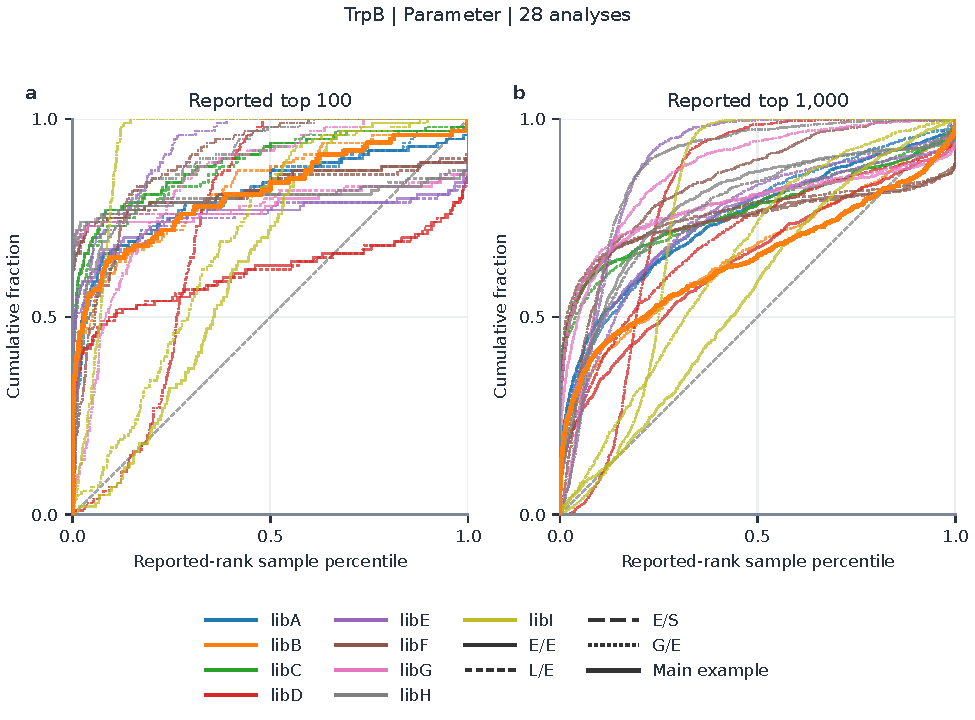
\includegraphics[width=\linewidth]{reported_curves_parameter_posterior_trpb_01.pdf}
\caption{TrpB reported-rank percentile curves: parameter. Each of the 28 lines per panel is one landscape/model analysis; panels use the reported top 100 and top 1000. Colors identify landscapes and line styles identify models. E, L, and G denote Exponential, Lomax, and Gamma priors; a second E or S denotes exponential or sigmoid growth. A thicker line marks the main example. All percentiles are retained; curves are overlaid, not averaged or pooled. Table~\ref{tab:reported-curve-statistics} gives each analysis's area, correlation, and counts. The gray diagonal is descriptive, not a calibration target.}
\label{fig:curves-parameter_posterior-trpb-1}
\end{figure}
\clearpage

\begin{figure}[p]
\centering
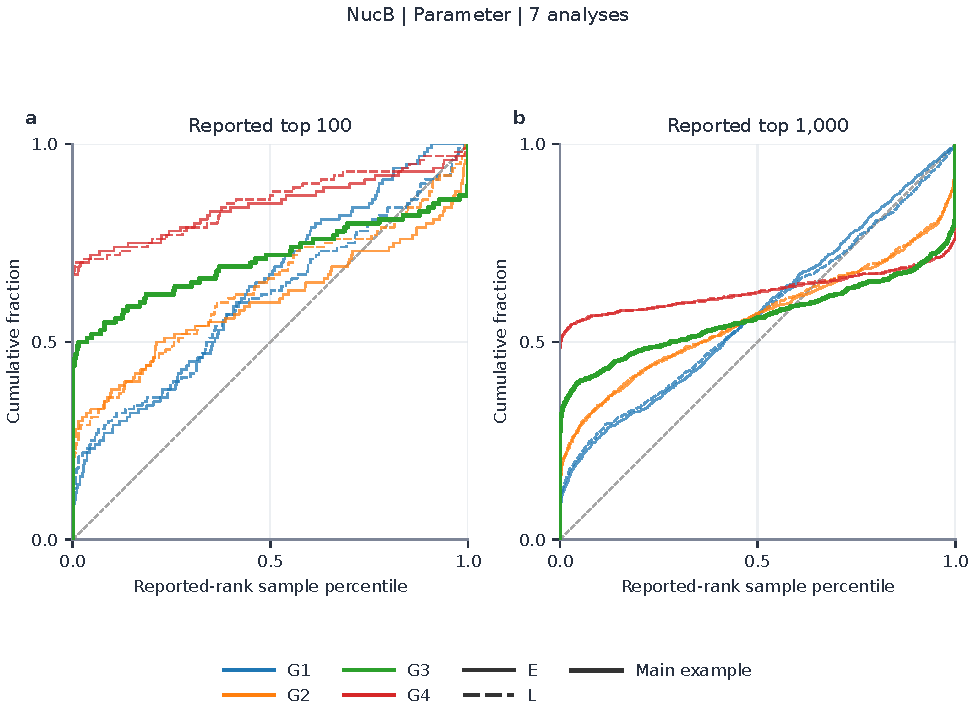
\includegraphics[width=\linewidth]{reported_curves_parameter_posterior_nuc_01.pdf}
\caption{NucB reported-rank percentile curves: parameter. Each of the 7 lines per panel is one landscape/model analysis; panels use the reported top 100 and top 1000. Colors identify landscapes and line styles identify models. E, L, and G denote Exponential, Lomax, and Gamma priors; a second E or S denotes exponential or sigmoid growth. A thicker line marks the main example. All percentiles are retained; curves are overlaid, not averaged or pooled. Table~\ref{tab:reported-curve-statistics} gives each analysis's area, correlation, and counts. The gray diagonal is descriptive, not a calibration target.}
\label{fig:curves-parameter_posterior-nuc-1}
\end{figure}
\clearpage

\begin{figure}[p]
\centering
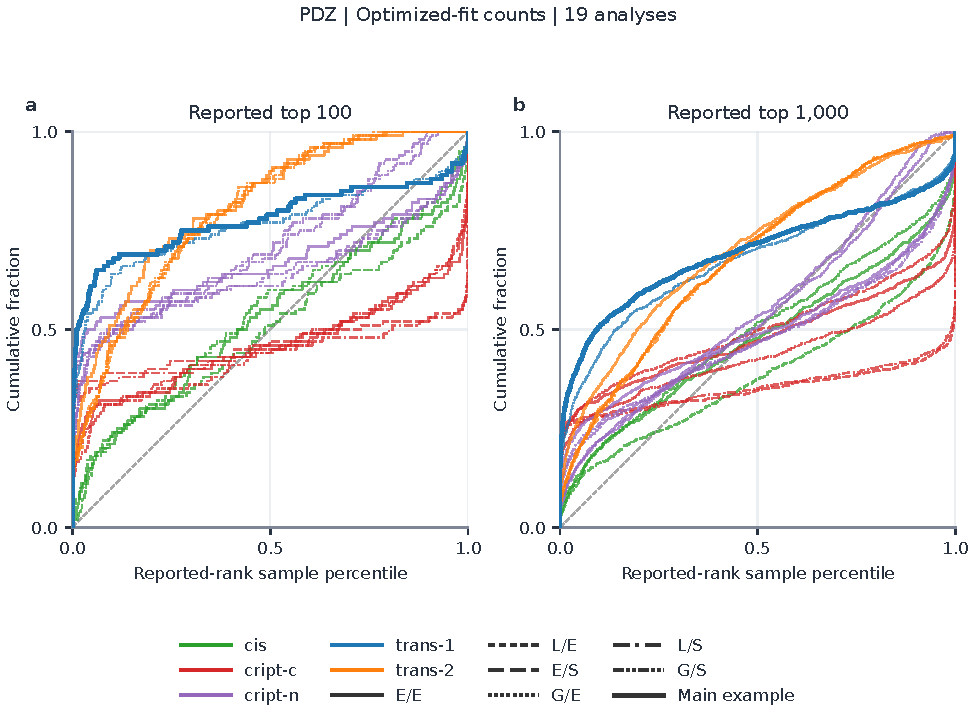
\includegraphics[width=\linewidth]{reported_curves_mle_predictive_pdz_01.pdf}
\caption{PDZ reported-rank percentile curves: optimized-fit counts. Each of the 19 lines per panel is one landscape/model analysis; panels use the reported top 100 and top 1000. Colors identify landscapes and line styles identify models. E, L, and G denote Exponential, Lomax, and Gamma priors; a second E or S denotes exponential or sigmoid growth. A thicker line marks the main example. All percentiles are retained; curves are overlaid, not averaged or pooled. Table~\ref{tab:reported-curve-statistics} gives each analysis's area, correlation, and counts. The gray diagonal is descriptive, not a calibration target.}
\label{fig:curves-mle_predictive-pdz-1}
\end{figure}
\clearpage

\begin{figure}[p]
\centering
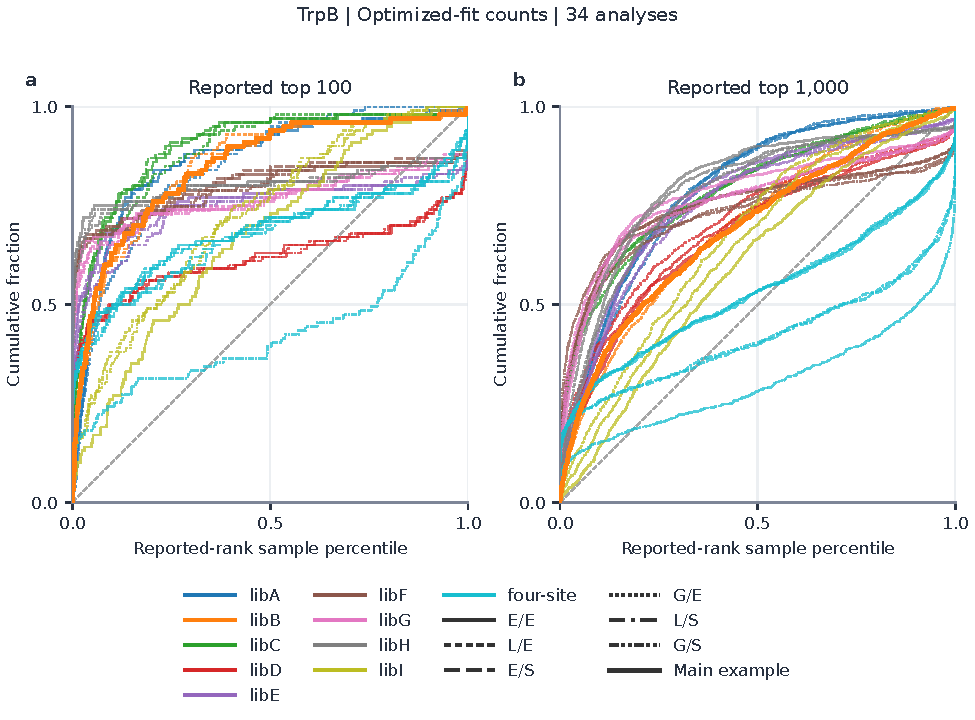
\includegraphics[width=\linewidth]{reported_curves_mle_predictive_trpb_01.pdf}
\caption{TrpB reported-rank percentile curves: optimized-fit counts. Each of the 34 lines per panel is one landscape/model analysis; panels use the reported top 100 and top 1000. Colors identify landscapes and line styles identify models. E, L, and G denote Exponential, Lomax, and Gamma priors; a second E or S denotes exponential or sigmoid growth. A thicker line marks the main example. All percentiles are retained; curves are overlaid, not averaged or pooled. Table~\ref{tab:reported-curve-statistics} gives each analysis's area, correlation, and counts. The gray diagonal is descriptive, not a calibration target.}
\label{fig:curves-mle_predictive-trpb-1}
\end{figure}
\clearpage

\begin{figure}[p]
\centering
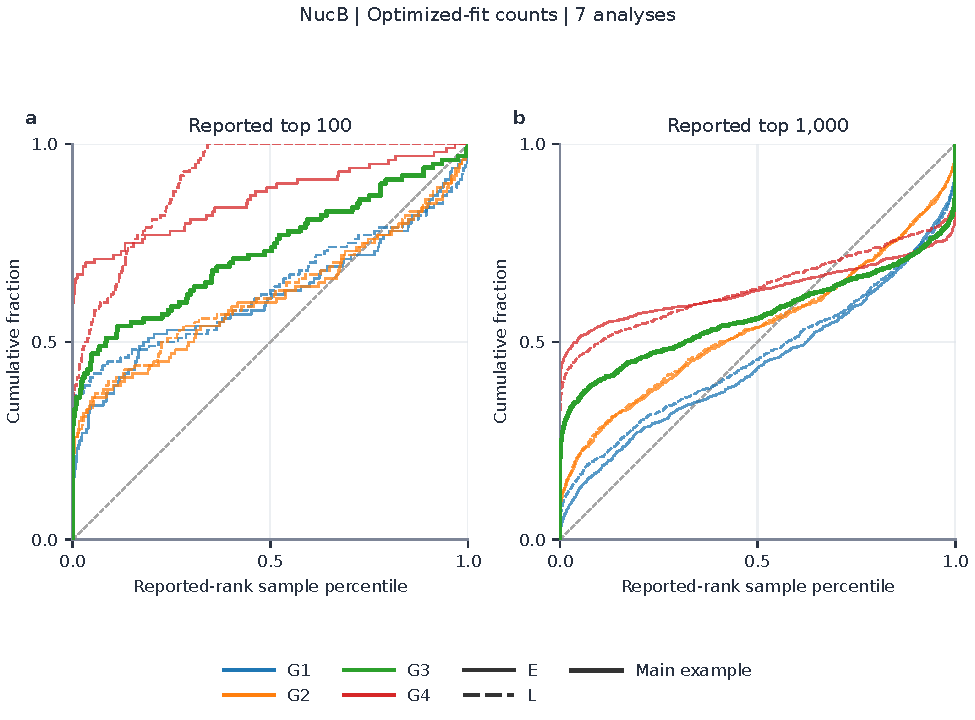
\includegraphics[width=\linewidth]{reported_curves_mle_predictive_nuc_01.pdf}
\caption{NucB reported-rank percentile curves: optimized-fit counts. Each of the 7 lines per panel is one landscape/model analysis; panels use the reported top 100 and top 1000. Colors identify landscapes and line styles identify models. E, L, and G denote Exponential, Lomax, and Gamma priors; a second E or S denotes exponential or sigmoid growth. A thicker line marks the main example. All percentiles are retained; curves are overlaid, not averaged or pooled. Table~\ref{tab:reported-curve-statistics} gives each analysis's area, correlation, and counts. The gray diagonal is descriptive, not a calibration target.}
\label{fig:curves-mle_predictive-nuc-1}
\end{figure}
\clearpage

\begin{figure}[p]
\centering
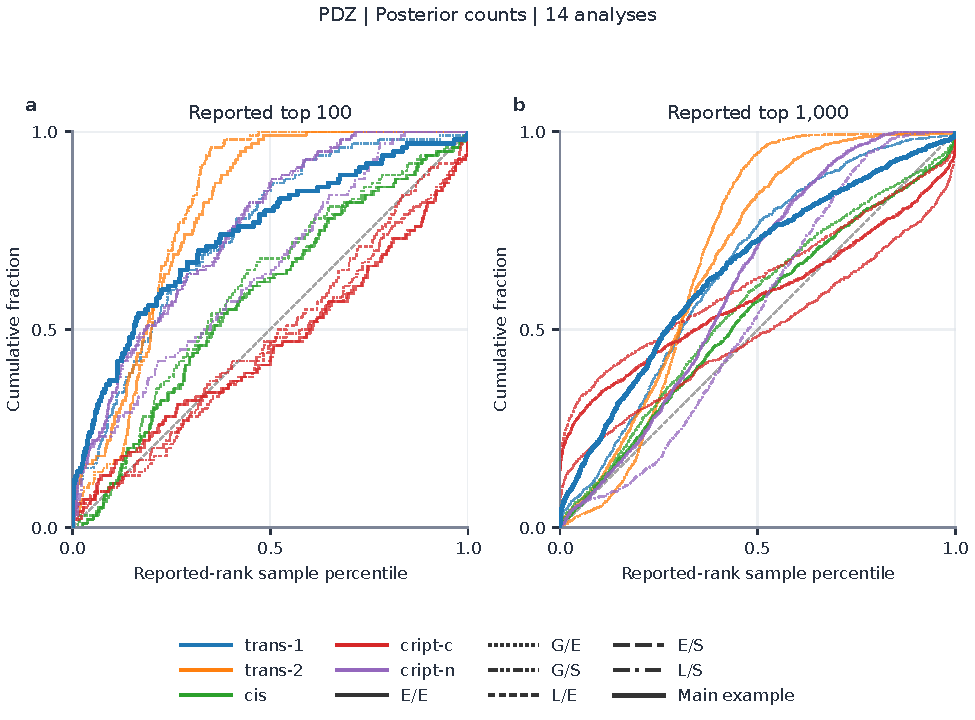
\includegraphics[width=\linewidth]{reported_curves_posterior_predictive_pdz_01.pdf}
\caption{PDZ reported-rank percentile curves: posterior counts. Each of the 14 lines per panel is one landscape/model analysis; panels use the reported top 100 and top 1000. Colors identify landscapes and line styles identify models. E, L, and G denote Exponential, Lomax, and Gamma priors; a second E or S denotes exponential or sigmoid growth. A thicker line marks the main example. All percentiles are retained; curves are overlaid, not averaged or pooled. Table~\ref{tab:reported-curve-statistics} gives each analysis's area, correlation, and counts. The gray diagonal is descriptive, not a calibration target.}
\label{fig:curves-posterior_predictive-pdz-1}
\end{figure}
\clearpage

\begin{figure}[p]
\centering
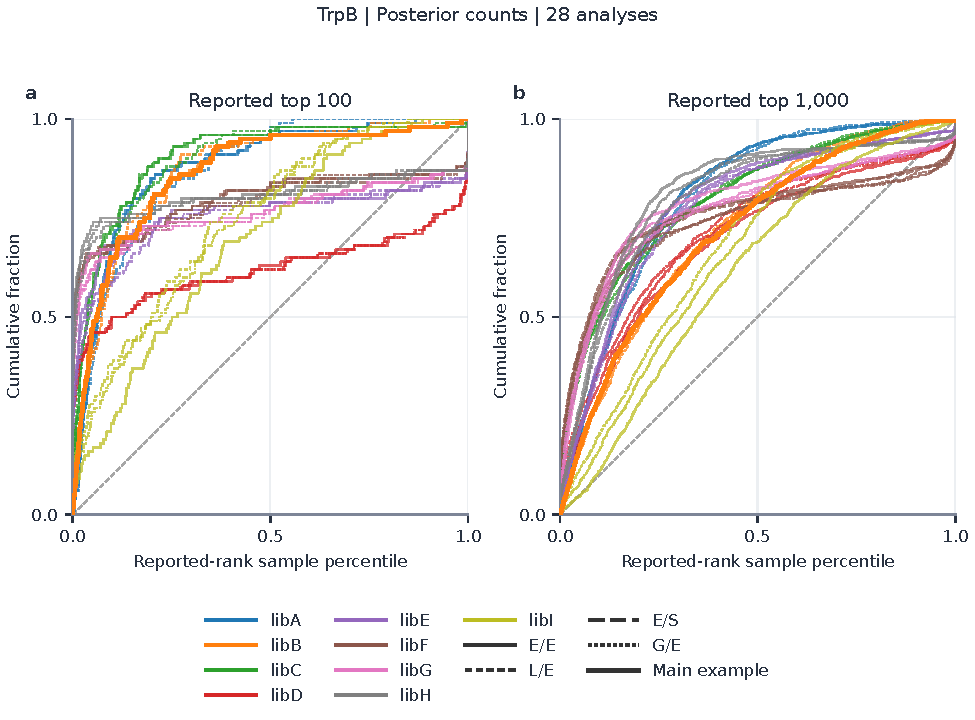
\includegraphics[width=\linewidth]{reported_curves_posterior_predictive_trpb_01.pdf}
\caption{TrpB reported-rank percentile curves: posterior counts. Each of the 28 lines per panel is one landscape/model analysis; panels use the reported top 100 and top 1000. Colors identify landscapes and line styles identify models. E, L, and G denote Exponential, Lomax, and Gamma priors; a second E or S denotes exponential or sigmoid growth. A thicker line marks the main example. All percentiles are retained; curves are overlaid, not averaged or pooled. Table~\ref{tab:reported-curve-statistics} gives each analysis's area, correlation, and counts. The gray diagonal is descriptive, not a calibration target.}
\label{fig:curves-posterior_predictive-trpb-1}
\end{figure}
\clearpage

\begin{figure}[p]
\centering
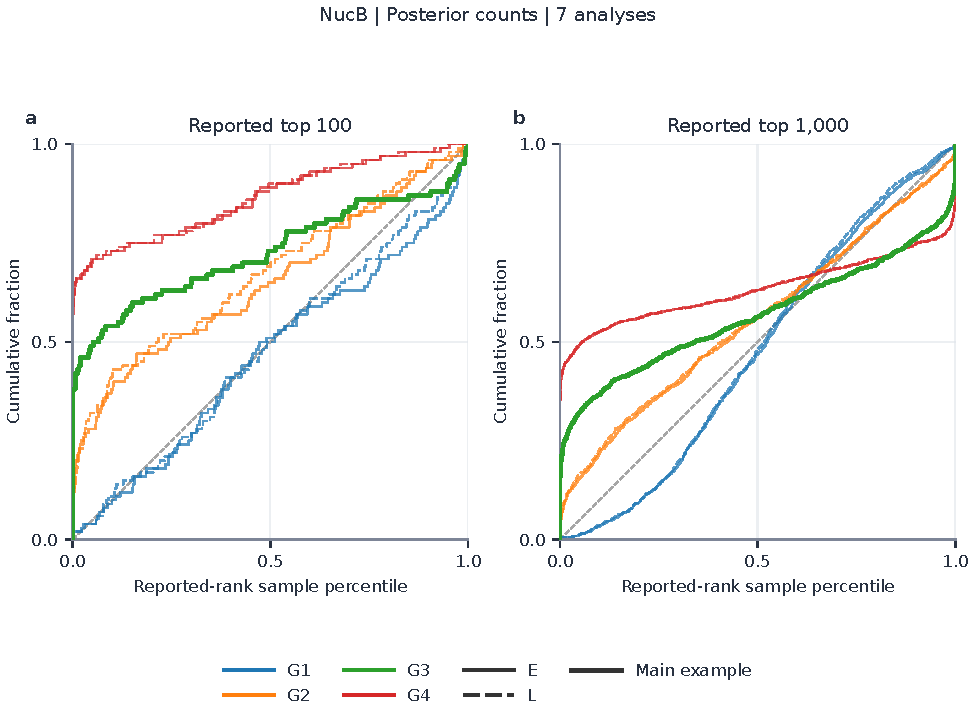
\includegraphics[width=\linewidth]{reported_curves_posterior_predictive_nuc_01.pdf}
\caption{NucB reported-rank percentile curves: posterior counts. Each of the 7 lines per panel is one landscape/model analysis; panels use the reported top 100 and top 1000. Colors identify landscapes and line styles identify models. E, L, and G denote Exponential, Lomax, and Gamma priors; a second E or S denotes exponential or sigmoid growth. A thicker line marks the main example. All percentiles are retained; curves are overlaid, not averaged or pooled. Table~\ref{tab:reported-curve-statistics} gives each analysis's area, correlation, and counts. The gray diagonal is descriptive, not a calibration target.}
\label{fig:curves-posterior_predictive-nuc-1}
\end{figure}
\clearpage
